\begin{figure}[H]
\centering
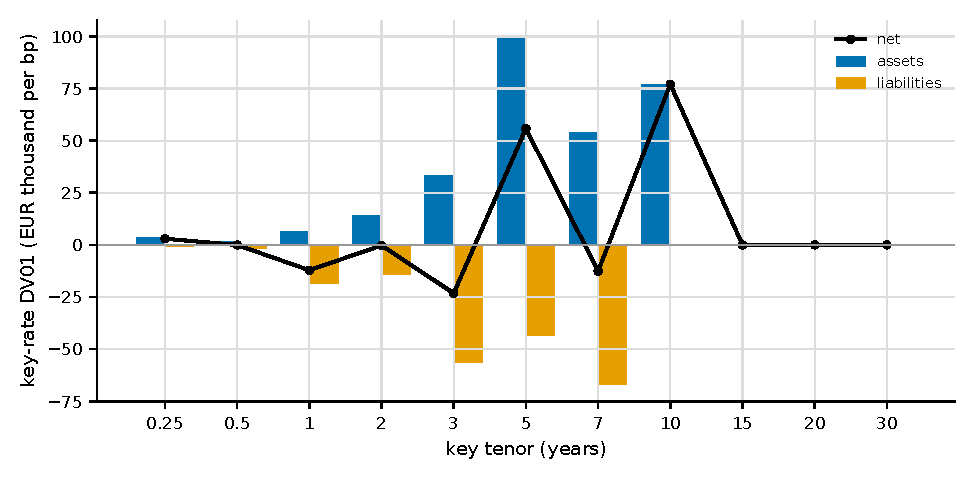
\includegraphics[width=\linewidth]{figures/fig15_key_rates.pdf}
\caption{Key-rate DV01 profile of the reference bank: value change for a 1 bp fall of the zero curve around each key tenor (tent-shaped bumps; the key rates sum to the parallel DV01). Assets gain, liabilities (negative cash flows) lose when rates fall; the net line is the bank's exposure.}
\label{fig:fig15_key_rates}
\end{figure}
